\section[Workflow]{Skills and an end-to-end workflow}
\sectionframe{06}{Skills and an end-to-end workflow}
  {How does a request become a reviewed change?}
  {\faProjectDiagram}

% ------------------------------------------------------------ what a skill is
% a lab protocol beside a skill file, row for row: what it is called, when to use it, the steps
\begin{frame}[source={Pocock (2026), mattpocock/skills v1.3.1: tdd · agentskills.io, Specification}]{A skill: a lab protocol for the agent}
  \begin{tikzpicture}[x=1mm,y=1mm,
      head/.style={anchor=north west,inner sep=0pt,font=\small\bfseries,text=udsdark},
      prot/.style={anchor=base west,inner sep=0pt,font=\footnotesize,text=udsdark},
      code/.style={anchor=base west,inner sep=0pt,font=\ttfamily\fontsize{7.2}{8.4}\selectfont,text=udsdark},
      num/.style={circle,fill=udsblue,text=white,inner sep=0pt,minimum size=3.6mm,
        font=\fontsize{7}{7}\selectfont\bfseries},
      pair/.style={udsgreymid,line width=0.5pt,dash pattern=on 1pt off 1pt},
      key/.style={fill=white,inner xsep=0.8mm,inner ysep=0.3mm,font=\scriptsize,text=udsgrey},
      say/.style={anchor=north west,inner sep=0pt,font=\scriptsize,text=udsdark}]
    \useasboundingbox (0,0) rectangle (144,-54);
    \node[head] at (0,0) {In the lab\enspace{\mdseries\color{udsgrey}a protocol}};
    \node[head] at (76,0) {In the repository\enspace{\mdseries\color{udsgrey}a skill}};
    % the protocol: a sheet on a clipboard
    \draw[udsgreylight,fill=white,line width=0.5pt,rounded corners=1.2mm] (0,-5.6) rectangle (62,-43.6);
    \fill[udsgreymid,rounded corners=0.8mm] (24,-4.3) rectangle (38,-7.1);
    \node[prot,font=\footnotesize\bfseries] at (3,-14.6) {Sample preparation};
    \node[prot,text=udsgrey] at (3,-18.6) {Use when: a specimen goes to the SEM.};
    \foreach \t [count=\i] in {Grind.,Polish.,Etch.,Check under the light microscope.} {
      \pgfmathsetmacro\y{-29-(\i-1)*4}
      \node[num] at (4.8,\y+0.95) {\i};
      \node[prot] at (8.4,\y) {\t};
    }
    % the skill: its SKILL.md in a file window, as on the slides of section 4
    \node[anchor=north west,inner xsep=1.8mm,inner ysep=0.8mm,text height=1.9mm,text depth=0.6mm,
      font=\ttfamily\fontsize{7}{8}\selectfont,text=udsdark] (tab) at (76,-5.6)
      {\textcolor{udsblue}{\faIcon[regular]{file-alt}}\enspace tdd/SKILL.md\enspace
       \textcolor{udsgreymid}{\sffamily\scriptsize abridged}};
    \begin{scope}
      \clip[rounded corners=1.2mm] (76,-5.6) rectangle (144,-43.6);
      \fill[darktint] (tab.north east) rectangle (144,-9.7);
      \draw[udsblue,line width=0.9pt] (tab.north west) -- (tab.north east);
    \end{scope}
    \draw[udsgreylight,line width=0.5pt,rounded corners=1.2mm] (76,-5.6) rectangle (144,-43.6);
    \node[code] at (78.8,-14.6) {name: tdd};
    \node[code] at (78.8,-18.6) {description: Test-driven development. Use when};
    \node[code] at (78.8,-21.6) {\phantom{xx}the user wants to build features or fix};
    \node[code] at (78.8,-24.6) {\phantom{xx}bugs test-first, ...};
    \foreach \t [count=\i] in {Agree the seams to test.,Write one failing test.,
        Write just enough code to pass.,Repeat for the next behaviour.}
      \node[code] at (78.8,{-29-(\i-1)*4}) {\i. \t};
    % what matches what, the word on its line
    \foreach \y/\k in {-13.7/name,-17.7/when,-34.6/steps} {
      \draw[pair] (63.2,\y) -- (74.8,\y);
      \node[key] at (69,\y) {\k};
    }
    \node[say] at (0,-45.6) {written once; everyone in the lab follows it};
    \node[say] at (76,-45.6) {written once; the agent follows it when needed};
    \node[anchor=north west,inner sep=0pt,font=\footnotesize\bfseries,text=udsblue] at (0,-50.4)
      {one procedure per kind of task: worth writing when the task recurs};
  \end{tikzpicture}
  \note{\textbf{25:00--26:00}\par
    Section 4 gave the agent facts about the repository; a skill gives it a procedure.\par
    It works like a lab protocol: a name, when to use it, and the steps, written once and
      followed by whoever does the task.\par
    A skill is the same for an agent: a Markdown file, here an abridged version of Pocock's
      test-driven development skill.\par
    Without one, we type the same instructions into every prompt, a little differently each
      time.\par
    Written once, the procedure is kept with the project, reviewed like code and improved in one
      place.\par
    Worth it for a task that recurs; a one-off task needs only a good prompt.}
\end{frame}

% ------------------------------------------------------------ inside a skill
\begin{frame}[fragile,source={Pocock (2026), mattpocock/skills v1.3.1: tdd · agentskills.io, Specification · Anthropic (2026), Claude Code docs: Skills · OpenAI (2026), Build skills}]{Skills: procedures loaded when needed}
  \begin{columns}[T,onlytextwidth]
    \begin{column}{0.57\textwidth}
\begin{codefile}[basicstyle=\ttfamily\fontsize{7}{8.4}\selectfont]{tdd/SKILL.md\enspace\textcolor{udsgreymid}{\sffamily\scriptsize abridged}}
---
name: tdd
description: Test-driven development. Use when the user
  wants to build features or fix bugs test-first,
  mentions "red-green-refactor", or wants integration
  tests.
---
# Test-Driven Development
## What a good test is
Tests verify behavior through public interfaces, not
implementation details. ...
See [tests.md](tests.md) for examples and
[mocking.md](mocking.md) for mocking guidelines.
\end{codefile}
    \end{column}
    \begin{column}{0.4\textwidth}
      % one bracket per part of the file, level with its lines; y = 0 is the top of the file window
      \begin{tikzpicture}[x=1mm,y=1mm,
          what/.style={anchor=west,inner sep=0pt,font=\footnotesize,text=udsdark,align=left,text width=52mm,
            execute at begin node={\hyphenpenalty=10000\raggedright}}]
        \useasboundingbox (0,0) rectangle (57.6,-54);
        \def\first{6.6}\def\pitch{2.952}% the first line's top below the window's top, and the line pitch
        \foreach \a/\b/\t in {1/7/{\textcolor{udsblue}{\bfseries from the start}, like \fn{AGENTS.md}\\
              the name and description of every skill},
            8/11/{\textbf{when it runs}\\ \fn{/tdd}, or a task that matches},
            12/13/{\textbf{when the steps need them}\\ \fn{tests.md}, \fn{mocking.md} in the same folder}} {
          \pgfmathsetmacro\ya{-\first-(\a-1)*\pitch-0.5}
          \pgfmathsetmacro\yb{-\first-\b*\pitch+0.5}
          \draw[udsgreymid,line width=0.6pt] (0,\ya) -- (1.4,\ya) -- (1.4,\yb) -- (0,\yb);
          \node[what] at (3.6,{(\ya+\yb)/2}) {\t};
        }
        \node[anchor=north west,inner sep=0pt,font=\scriptsize,text=udsgrey,text width=56mm,align=left]
          at (0,-48.4) {\textcolor{udsblue}{\faFolderOpen}\enspace\fn{.claude/skills/} (Claude Code),
          \fn{.agents/skills/} (Codex)};
      \end{tikzpicture}
    \end{column}
  \end{columns}
  \note{\textbf{26:00--27:10}\par
    Technically, a skill is a folder with a SKILL.md file and, where needed, more files beside
      it.\par
    The file starts with a name and a description, which says what the skill is for and when to
      use it.\par
    At the start of a session the agent sees only these lines, for every installed skill, about a
      hundred tokens each, just as it always sees AGENTS.md.\par
    The rest of the file loads when the skill runs: when we type its name, here /tdd, or when the
      agent finds that a task matches the description.\par
    Files beside it, here examples of good tests and rules for mocks, are read only when the
      steps call for them; this is called progressive disclosure.\par
    Committed with the code, the skill reaches everyone who works in the repository.}
\end{frame}

% ------------------------------------------------------------ the collection
\begin{frame}[source={Pocock (2026), mattpocock/skills v1.3.1: README · github.com/mattpocock/skills, 20 Oct 2026}]{Pocock's skills: an open collection}
  \begin{columns}[T,onlytextwidth]
    \begin{column}{0.56\textwidth}
      % the repository's address, which the screenshot's crop leaves out, as a link
      {\footnotesize\href{https://github.com/mattpocock/skills}{\faGithub\enspace\underline{\fn{mattpocock/skills}}}\par}
      \vskip1.6mm
      \begin{tikzpicture}
        \node[anchor=south west,inner sep=0pt,draw=udsgreylight,line width=0.4pt] (img) at (0,0)
          {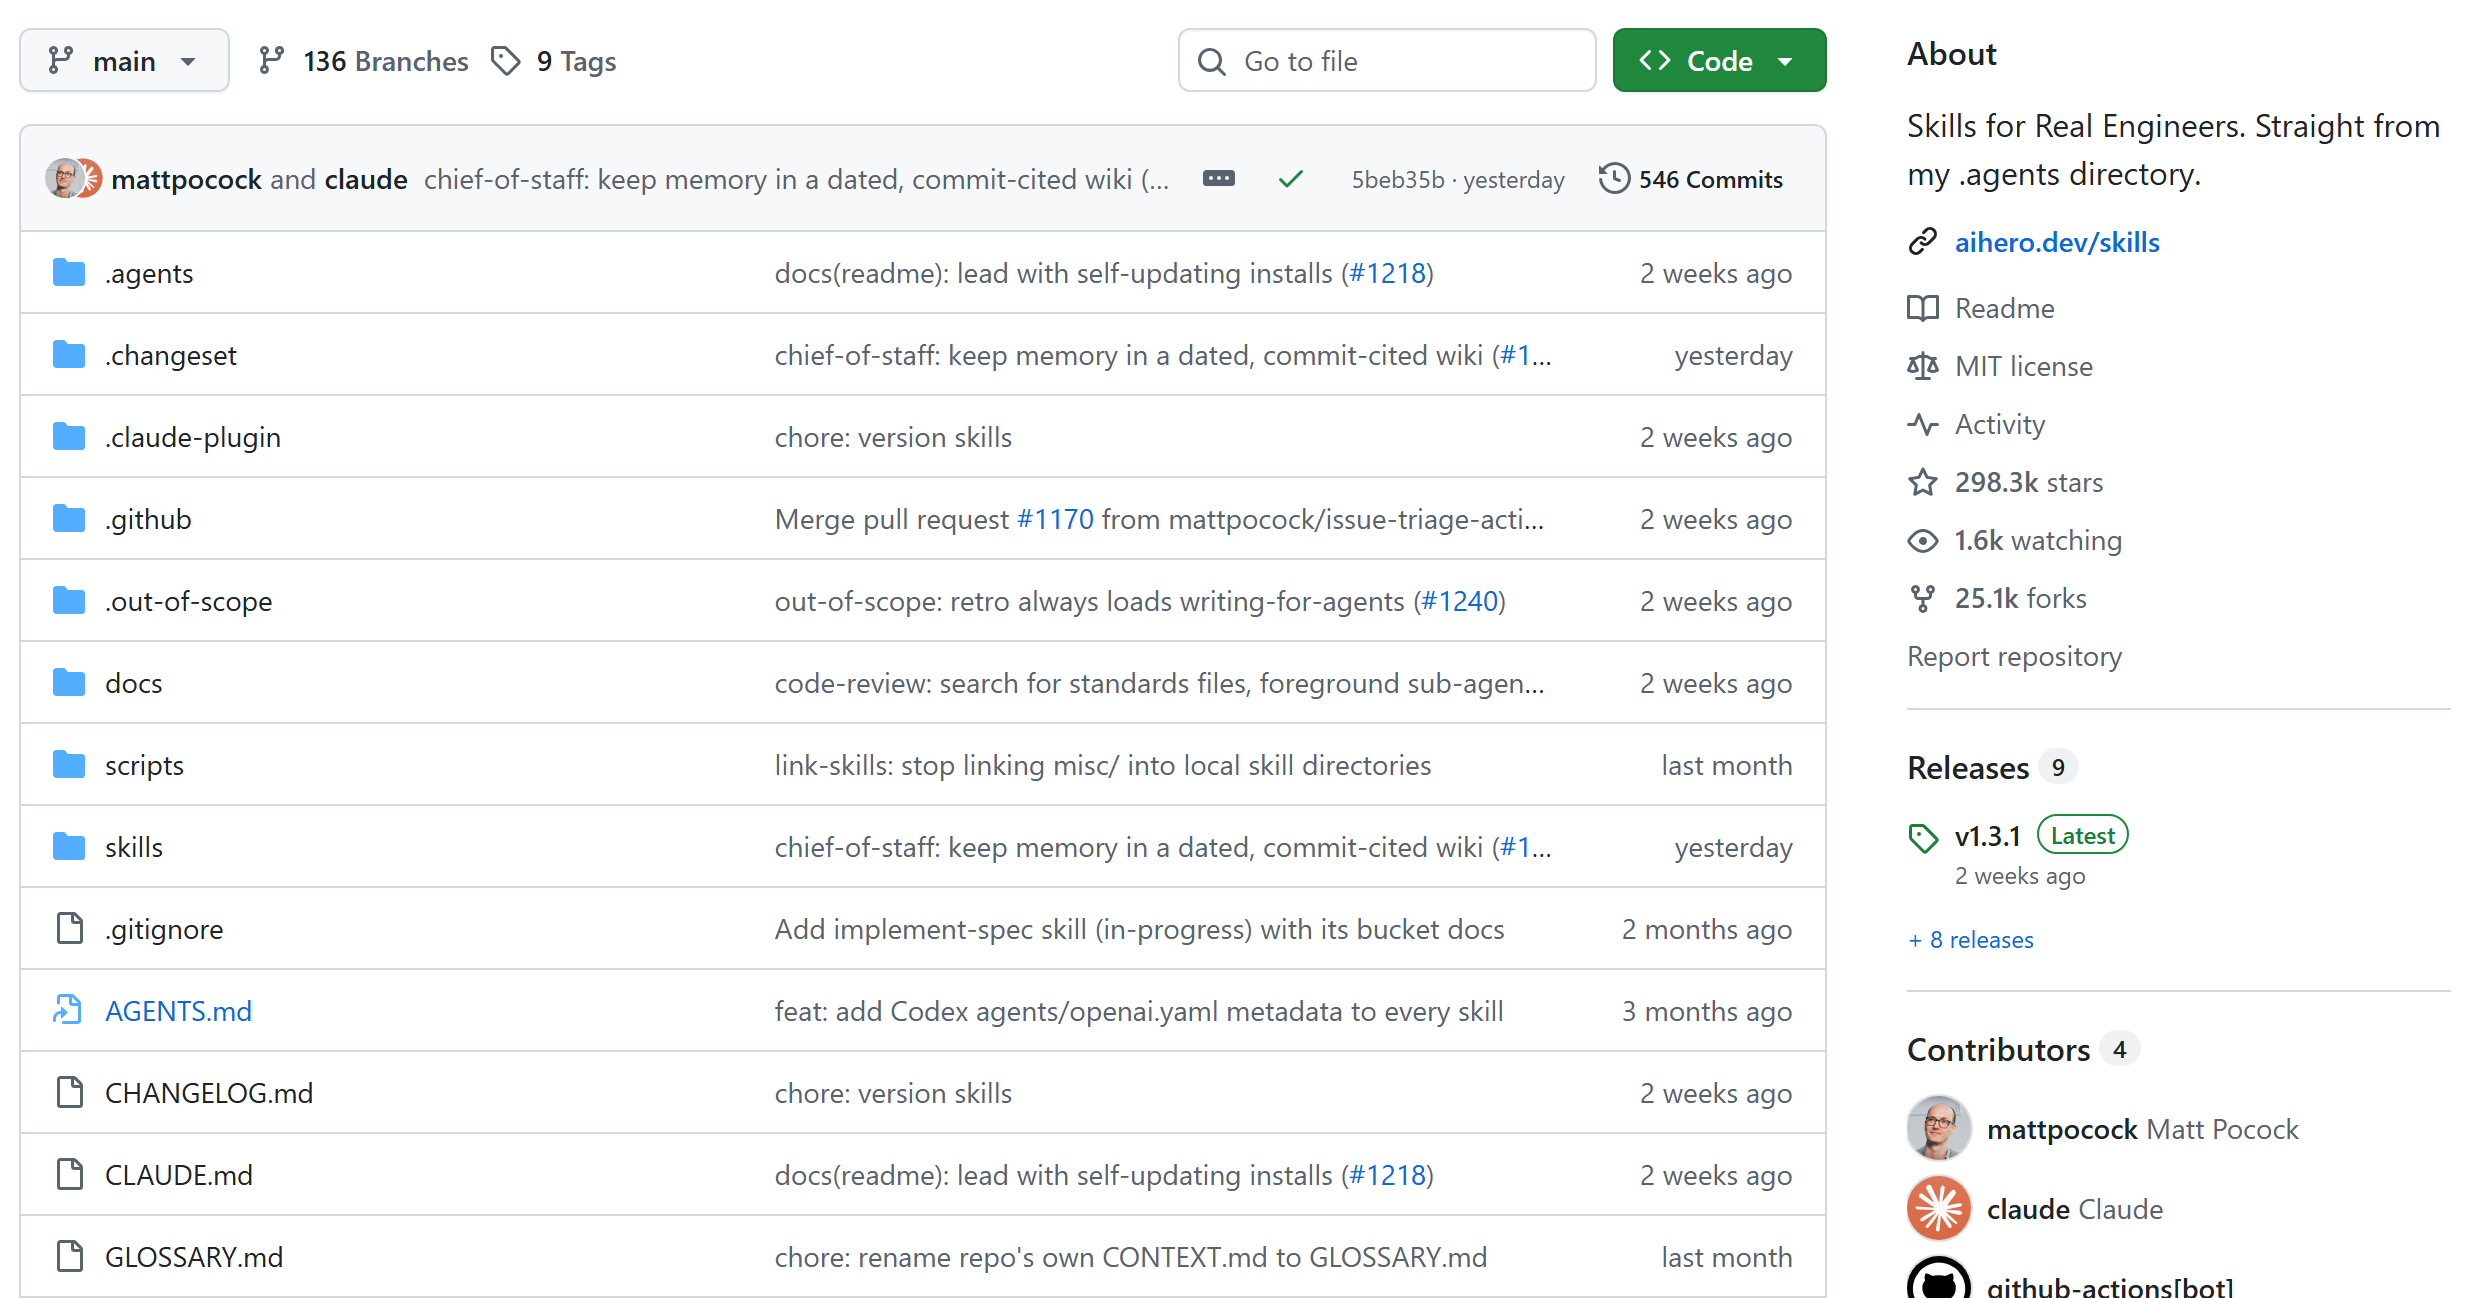
\includegraphics[width=\linewidth]{assets/screens/github-skills.png}};
        \begin{scope}[x={(img.south east)},y={(img.north west)},udsred,line width=1.1pt]
          \draw (0.014,0.320) rectangle (0.077,0.374);
          \draw (0.014,0.193) rectangle (0.109,0.247);
          \draw (0.014,0.005) rectangle (0.123,0.058);
          \draw (0.766,0.333) rectangle (0.871,0.386);
        \end{scope}
      \end{tikzpicture}\par\vskip1mm
      {\scriptsize\raggedright Boxed: \fn{skills/}, its own \fn{AGENTS.md} and \fn{GLOSSARY.md}, release v1.3.1.\par}
    \end{column}
    \begin{column}{0.41\textwidth}
      % two kinds of skill: the ones you type run a stage, and call the ones the agent may also pick
      \begin{tikzpicture}[x=1mm,y=1mm,
          kind/.style={anchor=north west,inner sep=0pt,font=\footnotesize\bfseries},
          chip/.style={anchor=west,minimum height=4.6mm,inner xsep=1mm,inner ysep=0pt,line width=0.5pt,
            font=\ttfamily\fontsize{7}{8}\selectfont,text=udsdark},
          you/.style={chip,draw=udsred,fill=redtint,minimum width=23.6mm},
          it/.style={chip,draw=udsblue,fill=bluetint,minimum width=22mm},
          call/.style={-{Stealth[length=1.5mm,width=1.1mm]},line width=0.5pt,draw=udsdark},
          say/.style={anchor=north west,inner sep=0pt,font=\scriptsize,text=udsgrey}]
        \useasboundingbox (0,0) rectangle (59,-54);
        \node[kind,text=udsred] at (0,0) {\faUser\enspace you type};
        \node[kind,text=udsblue] at (31,0) {\faRobot\enspace the agent may use};
        \foreach \s [count=\i from 0] in {/grill-with-docs,/to-spec,/to-tickets,/implement}
          \node[you] (u\i) at (0,{-7.6-\i*6.4}) {\s};
        \foreach \s [count=\i from 0] in {domain-modeling,codebase-design,tdd,code-review}
          \node[it] (m\i) at (31,{-7.6-\i*6.4}) {\s};
        % who calls whom, as the SKILL.md files say
        \draw[call] (u0.east) -- (m0.west);
        \draw[call] (u3.east) -- (m2.west);
        \draw[call] (u3.east) -- (m3.west);
        \draw[call] (m2.east) to[out=0,in=0,looseness=1.6] (m1.east);
        \node[say] at (0,-31.6) {each runs one stage};
        \node[say] at (31,-31.6) {rules and vocabulary};
        % installing: the files are copied into the project
        \fill[termbg,rounded corners=1mm] (0,-37) rectangle (57,-45.8);
        \foreach \c [count=\i] in {termdot1,termdot2,termdot3} \fill[\c] (\i*2.3,-39.2) circle (0.7);
        \node[inner sep=0pt,font=\ttfamily\fontsize{7}{8}\selectfont,text=termdim] at (28.5,-39.2) {install};
        \node[anchor=west,inner sep=0pt,font=\ttfamily\fontsize{7}{8}\selectfont,text=termfg] at (1.8,-43.4)
          {\textcolor{termgreen}{\$} npx skills@latest add mattpocock/skills};
        \node[say,text=udsred] at (0,-47.6) {\faExclamationTriangle\enspace read them first; note the commit};
      \end{tikzpicture}
    \end{column}
  \end{columns}
  \note{\textbf{27:10--28:00}\par
    Our example is Matt Pocock's open-source collection on GitHub; the repository uses its own
      AGENTS.md and GLOSSARY.md.\par
    Its skills come in two kinds: the ones we type each run one stage of the work, and they call
      skills that the agent may also pick up by itself, which hold the rules.\par
    Grill-with-docs calls domain-modeling, implement calls tdd and code-review, and tdd looks up
      codebase-design for its vocabulary.\par
    The installer copies the files into the project; skills are instructions and scripts written
      by someone else, so read them and note the commit you installed.}
\end{frame}

% ------------------------------------------------------- the books behind
% \bookcover{x}{colour}{title}{author}{year}: a book seen from the front, 22 x 27 mm, its top-left
% corner at (x,0); the darker strip on the left is the spine
\newcommand\bookcover[5]{%
  \begin{scope}
    \clip[rounded corners=0.9mm] (#1,0) rectangle ++(22,-27);
    \fill[#2] (#1,0) rectangle ++(22,-27);
    \fill[black,opacity=0.22] (#1,0) rectangle ++(1.9,-27);
  \end{scope}
  \node[anchor=north west,inner sep=0pt,text width=17.6mm,align=left,font=\scriptsize\bfseries,
    text=white,execute at begin node={\hyphenpenalty=10000\raggedright}] at (#1+3,-2.6) {#3};
  \node[anchor=south west,inner sep=0pt,text width=17.6mm,align=left,font=\scriptsize,
    text=white!80!#2] at (#1+3,-2.4-22.2) {#4\\#5};}
\begin{frame}[source={Hunt \& Thomas (1999) · Beck (1999; 2002) · Fowler (1999) · Evans (2003) · Ousterhout (2018) · Pocock (2026), mattpocock/skills v1.3.1: README, code-review, codebase-design}]{Classic practice, adapted for agents}
  % each book, the idea the skills take from it, and the skills that carry it
  \begin{tikzpicture}[x=1mm,y=1mm,
      idea/.style={anchor=north west,inner sep=0pt,text width=22mm,align=left,font=\scriptsize,
        text=udsdark,execute at begin node={\hyphenpenalty=10000\raggedright}},
      sk/.style={spec skill},
      fl/.style={spec chip}]
    \useasboundingbox (0,0) rectangle (144,-54);
    \bookcover{0}{udsdark}{The Pragmatic Programmer}{Andrew Hunt,\\David Thomas}{1999}
    \bookcover{24.4}{udsblue}{Extreme Programming Explained}{Kent Beck}{1999}
    \bookcover{48.8}{udsdark}{Refactoring}{Martin Fowler}{1999}
    \bookcover{73.2}{testgreen}{Test-Driven Development: By Example}{Kent Beck}{2002}
    \bookcover{97.6}{udsblue}{Domain-Driven Design}{Eric Evans}{2003}
    \bookcover{122}{udsdark}{A Philosophy of Software Design}{John\\Ousterhout}{2018}
    \foreach \x/\t in {0/{no one knows exactly what they want},24.4/{user stories; invest in the design every day},
        48.8/{code smells},73.2/{red, green, refactor},97.6/{a ubiquitous language},122/{deep modules}}
      \node[idea] at (\x,-29.4) {\t};
    \node[sk] at (0,-39.6) {/grill-with-docs};
    \node[sk] at (24.4,-39.6) {/to-spec};
    \node[sk] at (48.8,-39.6) {/code-review};
    \node[sk] at (73.2,-39.6) {/tdd};
    \node[fl] at (97.6,-39.6) {GLOSSARY.md};
    \node[sk] at (97.6,-45.2) {/domain-modeling};
    \node[sk] at (122,-39.6) {/codebase-design};
    \node[anchor=north west,inner sep=0pt,font=\footnotesize,text=udsdark] at (0,-50.4)
      {Pocock's README: ``They're based on decades of engineering experience.''};
  \end{tikzpicture}
  \note{\textbf{28:00--29:10}\par
    None of this is new: Pocock's README says the skills rest on decades of engineering
      experience, and quotes the books.\par
    The Pragmatic Programmer: no one knows exactly what they want, so the agent asks before it
      builds; its tracer bullets return as the vertical slices of to-tickets.\par
    Kent Beck's Extreme Programming brought the user stories that to-spec writes into every spec,
      and the advice to invest in the design every day.\par
    Fowler's Refactoring catalogues code smells, which code-review looks for in every diff.\par
    Beck's red, green, refactor loop is the tdd skill, the subject of section 7.\par
    Evans: one ubiquitous language for people and code, our glossary; Ousterhout: deep modules,
      much behaviour behind a small interface.\par
    What is new is the reader: the model has read these books, so a term such as tracer bullets
      or red and green brings the whole practice into a skill in a few words.}
\end{frame}

% Pocock's README, section "Why These Skills Exist", word for word (mattpocock/skills, MIT licence;
% the same on main on 3 November 2026 as in v1.3.1), with its links and the aside on the commit of its example glossary dropped: notes pages of their
% own, outside the frame, so they follow slide 25's notes page and stay out of the audience PDF. A
% note outside a frame does not get the theme's note style, so each one sets it first.
\note{\parindent=0pt\parskip=1.1mm\raggedright\footnotesize
  \textbf{Slide 25, continued (1 of 5): Pocock's README, ``Why These Skills Exist''}\par
  I built these skills as a way to fix common failure modes I see with Claude Code, Codex, and other
    coding agents.\par
  \textbf{\#1: The Agent Didn't Do What I Want}\par
  \emph{``No-one knows exactly what they want''}\enspace--- David Thomas \& Andrew Hunt, The Pragmatic
    Programmer\par
  \textbf{The Problem}. The most common failure mode in software development is misalignment. You think
    the dev knows what you want. Then you see what they've built - and you realize it didn't understand
    you at all.\par
  This is just the same in the AI age. There is a communication gap between you and the agent. The fix
    for this is a \textbf{grilling session} - getting the agent to ask you detailed questions about what
    you're building.\par
  \textbf{The Fix} is to use: \fn{/grill-me} - for non-code uses; \fn{/grill-with-docs} - same as
    \fn{/grill-me}, but adds more goodies (see below).\par
  These are my most popular skills. They help you align with the agent before you get started, and
    think deeply about the change you're making. Use them \emph{every} time you want to make a
    change.}
\note{\parindent=0pt\parskip=1.1mm\raggedright\footnotesize
  \textbf{Slide 25, continued (2 of 5)}\par
  \textbf{\#2: The Agent Is Way Too Verbose}\par
  \emph{``With a ubiquitous language, conversations among developers and expressions of the code are
    all derived from the same domain model.''}\enspace--- Eric Evans, Domain-Driven-Design\par
  \textbf{The Problem}: At the start of a project, devs and the people they're building the software
    for (the domain experts) are usually speaking different languages.\par
  I felt the same tension with my agents. Agents are usually dropped into a project and asked to figure
    out the jargon as they go. So they use 20 words where 1 will do.\par
  \textbf{The Fix} for this is a shared language. It's a document that helps agents decode the jargon
    used in the project.\par
  Example: here's an example glossary, from my \fn{course-video-manager} repo. Which one is easier to
    read? \textbf{BEFORE}: ``There's a problem when a lesson inside a section of a course is made `real'
    (i.e.\ given a spot in the file system)''. \textbf{AFTER}: ``There's a problem with the
    materialization cascade''. This concision pays off session after session.}
\note{\parindent=0pt\parskip=1.1mm\raggedright\footnotesize
  \textbf{Slide 25, continued (3 of 5)}\par
  \textbf{\#2, continued}\par
  This is built into \fn{/grill-with-docs}. It's a grilling session, but that helps you build a shared
    language with the AI, and document hard-to-explain decisions in ADR's.\par
  It's hard to explain how powerful this is. It might be the single coolest technique in this repo.
    Try it, and see.\par
  Tip: a shared language has many other benefits than reducing verbosity: \textbf{variables, functions
    and files are named consistently}, using the shared language; as a result, the \textbf{codebase is
    easier to navigate} for the agent; the agent also \textbf{spends fewer tokens on thinking}, because
    it has access to a more concise language.}
\note{\parindent=0pt\parskip=1.1mm\raggedright\footnotesize
  \textbf{Slide 25, continued (4 of 5)}\par
  \textbf{\#3: The Code Doesn't Work}\par
  \emph{``Always take small, deliberate steps. The rate of feedback is your speed limit. Never take on a
    task that's too big.''}\enspace--- David Thomas \& Andrew Hunt, The Pragmatic Programmer\par
  \textbf{The Problem}: Let's say that you and the agent are aligned on what to build. What happens when
    the agent \emph{still} produces crap?\par
  It's time to look at your feedback loops. Without feedback on how the code it produces actually runs,
    the agent will be flying blind.\par
  \textbf{The Fix}: You need the usual tranche of feedback loops: static types, browser access, and
    automated tests.\par
  For automated tests, a red-green-refactor loop is critical. This is where the agent writes a failing
    test first, then fixes the test. This helps give the agent a consistent level of feedback that
    results in far better code.\par
  I've built a \textbf{\fn{/tdd} skill} you can slot into any project. It encourages red-green-refactor
    and gives the agent plenty of guidance on what makes good and bad tests.\par
  For debugging, I've also built a \textbf{\fn{/diagnosing-bugs}} skill that wraps best debugging
    practices into a disciplined loop, gated phase by phase.}
\note{\parindent=0pt\parskip=1.1mm\raggedright\footnotesize
  \textbf{Slide 25, continued (5 of 5)}\par
  \textbf{\#4: We Built A Ball Of Mud}\par
  \emph{``Invest in the design of the system \emph{every day}.''}\enspace--- Kent Beck, Extreme Programming
    Explained\par
  \emph{``The best modules are deep. They allow a lot of functionality to be accessed through a simple
    interface.''}\enspace--- John Ousterhout, A Philosophy Of Software Design\par
  \textbf{The Problem}: Most apps built with agents are complex and hard to change. Because agents can
    radically speed up coding, they also accelerate software entropy. Codebases get more complex at an
    unprecedented rate.\par
  \textbf{The Fix} for this is a radical new approach to AI-powered development: caring about the design
    of the code.\par
  This is built in to every layer of these skills: \fn{/to-spec} quizzes you about which modules you're
    touching before creating a spec.\par
  And crucially, \fn{/improve-codebase-architecture} surveys a codebase for deepening opportunities and
    hands you the candidates. I recommend running it on your codebase once every few days. It is a
    survey, not a rescue: on a genuinely old codebase it will find real candidates, but it won't
    untangle the mud for you.\par
  \textbf{Summary}: Software engineering fundamentals matter more than ever. These skills are my best
    effort at condensing these fundamentals into repeatable practices, to help you ship the best apps of
    your career. Enjoy.}

% ------------------------------------------------------------ flow diagram
\begin{frame}[source={Pocock (2026), mattpocock/skills v1.3.1 · aihero.dev/skills}]{Pocock's flow: who does what}
  \begin{tikzpicture}[x=1mm,y=1mm,
      cell/.style={minimum width=24.4mm,text width=23.2mm,inner sep=0.6mm,align=center,
        execute at begin node={\hyphenpenalty=10000}},
      hcell/.style={cell,human,minimum height=9.6mm,font=\fontsize{7}{8}\selectfont},
      acell/.style={cell,agent,minimum height=17mm,font=\fontsize{7}{8}\selectfont},
      fcell/.style={cell,artifact,minimum height=7.6mm,font=\ttfamily\fontsize{7}{8}\selectfont},
      lane/.style={font=\fontsize{7}{8}\selectfont\bfseries,rotate=90,anchor=center,inner sep=0pt}]
    \node[lane,text=udsred]  at (3,-4.8)  {PERSON};
    \node[lane,text=udsblue] at (3,-23.5) {AGENT};
    \node[lane,text=udsdark] at (3,-39)   {OUTPUT};
    \foreach \skill/\act/\who/\res [count=\k from 0] in {
        grill-with-docs/{questions in rounds; updates the glossary}/{answer; settle the open points}/{GLOSSARY.md, ADR draft},
        to-spec/{writes the spec from the conversation}/{approve scope and acceptance}/{spec (file or issue)},
        to-tickets/{vertical slices, in order}/{approve slices and order}/{ticket files},
        implement/{drives /tdd at the agreed seams; runs the review; commits}/{confirm test seams; rerun the tests}/{code + tests, one commit},
        code-review/{standards and spec, in parallel; proposes refactoring}/{judge findings; review the science}/{report (in session)}} {
      \pgfmathsetmacro\x{20+\k*27.6}
      \node[hcell] (h\k) at (\x,-4.8) {\who};
      \node[acell] (a\k) at (\x,-23.5) {{\ttfamily\bfseries/\skill}\\[0.3mm]\act};
      \node[fcell] (f\k) at (\x,-39) {\res};
      % two-way: the person both steers the stage and decides on its output
      \draw[flow,{Stealth[length=1.7mm,width=1.3mm]}-{Stealth[length=1.7mm,width=1.3mm]},draw=udsred]
        (h\k.south) -- (a\k.north);
      \draw[flow] (a\k.south) -- (f\k.north);
    }
    \foreach \k [evaluate=\k as \n using int(\k+1)] in {0,...,3} \draw[flow,draw=udsblue] (a\k.east) -- (a\n.west);
    \node[artifact,anchor=north west,minimum width=134.6mm,minimum height=5mm,font=\scriptsize,inner sep=0.6mm]
      (ctx) at (7.8,-45.4) {read along the way:\enspace \texttt{AGENTS.md}\enspace\textperiodcentered\enspace
      \texttt{GLOSSARY.md}\enspace\textperiodcentered\enspace\texttt{docs/adr/}\enspace\textperiodcentered\enspace
      \texttt{CODING\_STANDARDS.md} (review)\enspace\textperiodcentered\enspace tests};
    \foreach \a/\b/\t in {7.8/87.4/{one session: clarify, specify, slice},
                          90.6/142.4/{a fresh session per ticket}} {
      \draw[udsgreymid,line width=0.5pt] (\a,-52.5) -- ++(0,-1.2) -- (\b,-53.7) -- ++(0,1.2);
      \node[lbl,anchor=north] at ({(\a+\b)/2},-54.1) {\t};
    }
  \end{tikzpicture}
  \note{\textbf{29:10--30:20}\par
    The main flow as the author documents it: clarify with grill-with-docs, write the spec, cut
      tickets, implement each ticket.\par
    In today's terms this is spec-driven development: an approved spec before any code, then each
      ticket built test-first.\par
    Tickets are vertical slices: each a thin path through the whole program, from the command
      line to the output, usable on its own.\par
    Implement drives the tdd skill at the test seams agreed in the spec, the public functions
      and command-line options that the tests call; then it runs code-review and commits.\par
    Code-review checks the repository's coding standards and the spec, and is where refactoring
      is proposed.\par
    Red marks the decisions that stay with us at every stage.\par
    The author's context advice: one session from clarification to tickets, then a fresh session
      per ticket that starts from the written ticket.}
\end{frame}

% ---------------------------------------------------- a grilling session
% \sessiondot{n}: a numbered marker, as on slide 13; \sessionmark{n} is the same without height, so a
% marker on a session line does not move the lines around it
\newcommand\sessiondot[1]{\tikz[baseline=-0.75ex]\node[circle,fill=udsred,text=white,inner sep=0pt,
  minimum size=3.6mm,font=\sffamily\fontsize{7}{7}\selectfont\bfseries] {#1};}
\newcommand\sessionmark[1]{\smash{\sessiondot{#1}}}
% \sessionarrow{text}: a session line, then an arrow from its end across the column gap to the
% window in the right column; drawn inside the frame, so the notes thumbnail shows it too. The
% terminal's text sits 3.2 mm inside its right edge (1 mm box separation plus 2.2 mm padding).
\newcommand\sessionarrow[1]{%
  \setbox0\hbox{\setbox2\hbox{x}\spaceskip=\wd2 #1}\copy0
  \edef\sessionarrowend{\the\dimexpr\linewidth+3.2mm+\colgap-\wd0+0.1mm\relax}%
  \tikz[overlay,baseline=0pt]\draw[udsred,line width=0.8pt,-{Stealth[length=2mm,width=1.6mm]}]
    (1.4mm,0.9mm) -- (\sessionarrowend,0.9mm);}
\begin{frame}[fragile,source={Pocock (2026), mattpocock/skills v1.3.1: grill-with-docs, grilling, domain-modeling · video of 16 Jul 2026}]{A \texttt{/grill-with-docs} session}
  % the gap between the columns, which the glossary arrow crosses
  \edef\colgap{\the\dimexpr0.03\textwidth\relax}
  \begin{columns}[T,onlytextwidth]
    \begin{column}{0.61\textwidth}
\begin{terminal}[basicstyle=\ttfamily\fontsize{7}{8}\selectfont]{example session}
> /grill-with-docs Add validation folds by specimen to the
  training CLI, as decided in ADR-0003.
§\textcolor{termred}{\smash{\faQuestionCircle}}§ §\textbf{Q1 Default number of folds}§: the manifest lists §\sessionmark{1}§
  three specimens. One fold per specimen?
§\textcolor{termblue}{\smash{\faArrowRight}}§ Yes: k = number of specimens; --folds can lower it. §\sessionmark{2}§

§\textcolor{termred}{\smash{\faQuestionCircle}}§ §\textbf{Q2 What validation claims}§: each specimen is the only
  one of its material state, a term GLOSSARY.md lacks.
  Report folds as unseen material states, and add it?
§\textcolor{termblue}{\smash{\faArrowRight}}§ Yes.

§\textcolor{termred}{\smash{\faQuestionCircle}}§ §\textbf{Q3 Rows without specimen\_id}§: stop with a ValueError,
  as CODING_STANDARDS.md asks?
§\textcolor{termblue}{\smash{\faArrowRight}}§ Yes, and name the rows in the message.
> yes to all
§\sessionarrow{Updated GLOSSARY.md: Material state.}§
No ADR: the number of folds is easy to change later. §\sessionmark{3}§
\end{terminal}
    \end{column}
    \begin{column}{0.36\textwidth}
      % the legend on top; the glossary window at the bottom, level with the line that updates it
      \begin{minipage}[t][58mm][t]{\linewidth}
        \footnotesize
        \begin{tabular}{@{}c@{\enspace}l@{}}
          \sessiondot{1} & a fact the agent looked up\\[1.4mm]
          \sessiondot{2} & a recommended answer\\[1.4mm]
          \sessiondot{3} & an ADR only if hard to reverse\\
        \end{tabular}
        \vfill
\begin{codefile}[basicstyle=\ttfamily\fontsize{7}{8}\selectfont]{GLOSSARY.md\enspace\textcolor{udsgreymid}{new entry}}
Material state: the processing
  condition of a specimen (AsCast,
  Q980_0h_WC, Q980_9h_AC); here,
  one specimen per state.
\end{codefile}
        \vspace{-2.2mm}% the box's own skip below it, so its bottom meets the terminal's
      \end{minipage}
    \end{column}
  \end{columns}
  \note{\textbf{30:20--31:40}\par
    What grilling looks like on our request; the session is abridged and written for our example
      in the format of Pocock's skills.\par
    Each round asks every question that can be asked now, numbered, each with a recommended
      answer (2), worded so that yes accepts it.\par
    The agent looks up facts itself, here the number of specimens in the manifest (1), and
      leaves the decisions to us.\par
    When a term settles, it goes into the glossary at once (the arrow); here the session finds
      that every specimen is also the only one of its material state, which matters for what
      validation can claim.\par
    It offers an ADR only when a decision is hard to reverse, surprising and a real trade-off,
      so the number of folds gets none (3).\par
    Pocock's video of July 2026 shows a full session on his own project.}
\end{frame}

% ------------------------------------------------------------- walkthrough
% \stagefile{node}{x centre}{y top}{tab}{body}: a small file window under a stage, drawn as the
% codefile box is; (node) is its page and (nodet) its tab
\newcommand\stagefile[5]{%
  \node[anchor=north west,inner xsep=1mm,inner ysep=0.7mm,text height=1.9mm,text depth=0.5mm,
    font=\ttfamily\fontsize{7}{8}\selectfont,text=udsdark] (#1t) at (#2-12.2,#3)
    {\textcolor{udsblue}{\faIcon[regular]{file-alt}}\enspace#4};
  \node[anchor=north,minimum width=24.4mm,text width=22mm,inner xsep=1.2mm,inner ysep=1.3mm,
    align=left,font=\ttfamily\fontsize{7}{8.4}\selectfont,text=udsdark] (#1) at (#2,#3-4.2) {#5};
  \begin{scope}
    \clip[rounded corners=1mm] (#2-12.2,#3) rectangle ($(#1.south)+(12.2,0)$);
    \fill[darktint] (#1t.north east) rectangle (#2+12.2,#3-4.2);
    \draw[udsblue,line width=1.4pt] (#1t.north west) -- (#1t.north east);
  \end{scope}
  \draw[udsgreylight,line width=0.5pt,rounded corners=1mm] (#2-12.2,#3) rectangle ($(#1.south)+(12.2,0)$);}
\begin{frame}{The specimen split, stage by stage}
  \begin{tikzpicture}[x=1mm,y=1mm,
      stage/.style={agent,minimum width=24.4mm,minimum height=6.2mm,inner sep=0.6mm,
        font=\ttfamily\bfseries\fontsize{7}{8}\selectfont},
      ticket/.style={draw=udsgreylight,fill=white,line width=0.5pt,anchor=north,minimum width=24.4mm,
        text width=21.4mm,inner xsep=1.5mm,inner ysep=0.9mm,align=left,font=\scriptsize,text=udsdark,
        execute at begin node={\hyphenpenalty=10000\raggedright},
        path picture={\fill[udsdark] (path picture bounding box.north west) rectangle
          ([xshift=0.9mm]path picture bounding box.south west);}},
      say/.style={anchor=north,inner sep=0pt,font=\scriptsize,text=udsgrey,align=center,text width=25mm,
        execute at begin node={\hyphenpenalty=10000}},
      commit/.style={circle,draw=udsblue,fill=white,line width=0.9pt,minimum size=3mm,inner sep=0pt}]
    % an invisible copy of a lane label of "Pocock's flow: who does what" gives this picture the
    % same left edge, so the five columns sit exactly under those of that slide
    \node[font=\fontsize{7}{8}\selectfont\bfseries,rotate=90,anchor=center,inner sep=0pt,opacity=0]
      at (3,-4.8) {PERSON};
    % the short request starts the flow
    \fill[termbg,rounded corners=1mm] (7.8,0) rectangle (142.6,-6.4);
    \foreach \c [count=\i] in {termdot1,termdot2,termdot3} \fill[\c] (7.8+\i*2.3,-3.2) circle (0.7);
    \node[anchor=west,inner sep=0pt,font=\ttfamily\fontsize{7}{8}\selectfont,text=termfg] at (17,-3.2)
      {> Add validation folds by specimen to the training CLI, as decided in ADR-0003.};
    % the five stages, as on "Pocock's flow: who does what"
    \foreach \s [count=\k from 0] in {grill-with-docs,to-spec,to-tickets,implement,code-review}
      \node[stage] (s\k) at (20+\k*27.6,-13.6) {/\s};
    \draw[flow] (20,-6.4) -- (s0.north);
    \foreach \k [evaluate=\k as \n using int(\k+1)] in {0,...,3} \draw[flow,draw=udsblue] (s\k.east) -- (s\n.west);
    \foreach \k in {0,...,4} \draw[flow] (s\k.south) -- ++(0,-3.4);
    % 1: answers, and a new glossary term
    \stagefile{w0}{20}{-21.2}{GLOSSARY.md}{\textcolor{testgreen}{+}\,Material state}
    \node[say] at ([yshift=-1.4mm]w0.south) {Q1 to Q3 answered};
    % 2: the spec
    \stagefile{w1}{47.6}{-21.2}{spec.md}{\textcolor{udsblue}{\bfseries\#\# Decisions}\\
      \textcolor{udsblue}{\bfseries\#\# Test seams}\\ \textcolor{udsblue}{\bfseries\#\# Out of scope}}
    % 3: three vertical slices, each usable on its own
    \node[ticket] (t1) at (75.2,-21.2) {\textbf{T1}\enspace\fn{--split specimen}, end to end};
    \node[ticket] (t2) at ([yshift=-1.4mm]t1.south) {\textbf{T2}\enspace overlap guard and errors};
    \node[ticket] (t3) at ([yshift=-1.4mm]t2.south) {\textbf{T3}\enspace provenance in the fold file};
    % 4: one commit per ticket, each in a fresh session
    \draw[udsblue,line width=1pt] (95.4,-20.4) -- (95.4,-45.6);
    \foreach \t [count=\i from 0] in {T1,T2,T3} {
      \node[commit] (k\i) at (95.4,-24-\i*8.6) {};
      \node[anchor=west,inner sep=0pt,font=\scriptsize,text=udsdark] at ([xshift=1.4mm]k\i.east)
        {\textbf{\t}\enspace tests, code};
    }
    \node[say] at (102.8,-47.6) {a fresh session per ticket};
    % 5: the review report on two axes
    \stagefile{w4}{130.4}{-21.2}{report}{\fontsize{7}{8.4}\sffamily
      \textcolor{udsblue}{\faSearch}\enspace standards\\[0.4mm] \textcolor{udsblue}{\faSearch}\enspace spec}
    \node[say] at ([yshift=-1.4mm]w4.south) {findings for you to judge};
  \end{tikzpicture}
  \note{\textbf{31:40--32:50}\par
    The whole flow on our task, starting from the short request.\par
    Each stage leaves something we can open and check.\par
    Grilling settles what the repository leaves open: the default number of folds, and what
      validation is meant to show with only three specimens.\par
    The spec records the decisions and the test seams.\par
    Tickets are thin vertical slices, each usable on its own: first the whole path from the
      command line to a fold file, then the overlap guard and the error cases, then the
      provenance stored in the fold file.\par
    Each ticket is implemented test-first in a fresh session, and review checks the standards
      and the spec.}
\end{frame}

% ---------------------------------------------------- when is it worth it
\begin{frame}[source={Pocock (2026), mattpocock/skills v1.3.1, ask-matt}]{When is the full flow worth it?}
  \centering
  \begin{tikzpicture}[x=1.55mm,y=1mm,pt/.style={circle,fill=udsdark,inner sep=0pt,minimum size=1.8mm}]
    \fill[bluetint] (0,0) rectangle (42,23);
    \fill[redtint] (42,23) rectangle (84,46);
    \draw[udsgreylight,line width=0.4pt] (42,0) -- (42,46) (0,23) -- (84,23);
    \draw[flow] (0,0) -- (86,0);
    \draw[flow] (0,0) -- (0,48);
    \node[lbl,anchor=north east,text=udsdark,font=\footnotesize] at (86,-0.8) {changes what a result means};
    \node[lbl,anchor=south,rotate=90,text=udsdark,font=\footnotesize] at (-0.8,24) {size and open questions};
    \node[lbl,anchor=south west,text=udsblue,font=\footnotesize\bfseries] at (1,1) {one prompt, review the diff};
    \node[lbl,anchor=north east,text=udsred,font=\footnotesize\bfseries] at (83,45) {grill, spec, tickets};
    \node[lbl,anchor=north west,text=udsdark,font=\footnotesize\bfseries] at (1,45) {slice it into tickets};
    \node[lbl,anchor=south east,text=udsdark,font=\footnotesize\bfseries] at (83,1) {write a short spec};
    \foreach \x/\y/\t in {7/9/fix a plot label, 14/16/add a CLI flag, 5/35/refactor the data loader,
        50/11/pixel-size units, 50/29/change the split unit, 60/38/new loss or metric} {
      \node[pt] (p) at (\x,\y) {};
      \node[lbl,anchor=west,text=udsdark,font=\scriptsize] at (p.east) {\t};
    }
  \end{tikzpicture}
  \note{\textbf{32:50--33:30}\par
    Not every change needs five stages.\par
    Two questions decide: how large or open is the change, and does it change what a result
      means?\par
    Small changes that leave results unchanged go straight to the agent; we still read the
      diff.\par
    A small change of meaning, such as pixel-size units, deserves a short spec.\par
    A large routine refactor benefits from tickets.\par
    The full flow earns its overhead when both hold, as for a new split unit, loss or
      metric.\par
    Pocock's own routing asks whether the build spans several sessions; the axis of meaning is
      ours.}
\end{frame}
